% ::setlocal makeprg=cd\ presentazione\ &&\ pdflatex\ -interaction=batchmode\ main.tex\ &&\ xdg-open\ main.pdf\ &

\section{Teoria}


\begin{frame}[t]{La Metrica di \Sh}

    \begin{equation*}
        \dd s^2 = - \left( 1 - \frac{2GM}{c^2r} \right) c^2 \dd t^2
        + \left( 1 - \frac{2GM}{c^2r} \right)^{-1} \dd r^2
        + r^2 (\dd \theta^2 + \sin^2 \theta \dd \phi^2)
    \end{equation*}

    Descrive uno spaziotempo stazionario e a simmetria sferica

    \begin{itemize}
        \item stella sferica
        \item buco nero
    \end{itemize}

    \begin{figure}
        \centering
        \includegraphics[width=0.5\textwidth]{Figures/ch1/sh.jpg}
        \caption{https://www.physicsforums.com/}%insights/wp-content/uploads/2017/12/Schwarzschild-Space.jpg
    \end{figure}

\end{frame}


\begin{frame}[t]{La Metrica di \Sh}

    \begin{equation*}
        \dd s^2 = - \left( 1 - \frac{2M}{r} \right) \dd t^2
        + \left( 1 - \frac{2M}{r} \right)^{-1} \dd r^2
        + r^2 (\dd \theta^2 + \sin^2 \theta \dd \phi^2)
    \end{equation*}
    
    %\begin{equation*}
    %    g_{\nu \mu} = 
    %    \begin{array}{cc}
    %        \begin{pNiceMatrix}[first-row,first-col][columns-width = 0.9cm]
    %              & t & r & \theta & \phi \\
    %            t~~ & - \left( 1 - \frac{2M}{r} \right) & 0 & 0 & 0 \\  
    %            r~~ & 0 & \frac{1}{\left( 1 - \frac{2M}{r} \right)} & 0 & 0 \\ 
    %            \theta~~ & 0 & 0 & r^2 & 0 \\
    %            \phi~~ & 0 & 0 & 0 & r^2 \sin^2 \theta \\
    %        \end{pNiceMatrix} &
    %    \end{array}
    %    \label{cap1:eq:Sh_g}
    %\end{equation*}

    \vspace{0.5cm}

    Unità geometriche: $\frac{GM}{c^2} \to G$, $ct \to t$

    \vspace{0.5cm}

    \begin{description}
        \item[$r = 0$] singolarità fisica \\
        \item[$r = 2M$] singolarità di coordinate \\
        \item[$r \to \infty$] metrica di \Mi \\
    \end{description}

\end{frame}


\subsection{Particelle di Test}

\begin{frame}[t]{La Metrica di \Sh}

    \begin{equation*}
        \dd s^2 = - \left( 1 - \frac{2M}{r} \right) \dd t^2
        + \left( 1 - \frac{2M}{r} \right)^{-1} \dd r^2
        + r^2 (\dd \theta^2 + \sin^2 \theta \dd \phi^2)
    \end{equation*}
    
    \vspace{0.5cm}

    \`E indipendente da $t$ e $\phi$ $\implies$ vettori di Killing associati
    
    \begin{equation*}
        \xi^\mu = \left( 1, 0, 0, 0 \right) \quad \eta^\mu = \left( 0, 0, 0, 1 \right)
    \end{equation*}

    Possiamo trovare delle costanti del moto

    \begin{align*}
        e &= - \mathbf{\xi \cdot u} = \left(1 - \frac{2M}{r} \right) \dv{t}{\tau} \\
        l &= \mathbf{\eta \cdot u} = r^2 \sin^2 \theta \dv{\phi}{\tau}
    \end{align*}

\end{frame}


\begin{frame}{L'Orbita Giace su un Piano}

    \begin{minipage}{0.49 \textwidth}

    % 3D AXIS with spherical coordinates
    \tdplotsetmaincoords{60}{110}
    \begin{tikzpicture}[scale=2,tdplot_main_coords]
      
        % Red vector coordinates
        \def\rvec{1.15}
        \def\thetavec{90}
        \def\phivec{70}
        
        % AXES
        \coordinate (O) at (0,0,0);
        \draw[thick,->] (0,0,0) -- (2,0,0) node[right=1]{$x$};
        \draw[thick,->] (0,0,0) -- (0,2,0) node[above=1]{$y$};
        \draw[thick,->] (0,0,0) -- (0,0,2) node[left=1]{$z$};
        
        % VECTORS
        \tdplotsetcoord{P}{\rvec}{\thetavec}{\phivec}
        \draw[thick,red] (O)  -- (P) node[below right]
            {$(r, \theta = \frac{\pi}{2}, \phi)$};
        %\draw[dashed]   (O)  -- (Pxy);
        \draw[dashed]   (P)  -- (Pxy);
        
        % ARCS
        \tdplotdrawarc[thick,->]{(O)}{0.4}{0}{\phivec} {anchor=north}{$\phi$}
        \tdplotsetthetaplanecoords{\phivec}
        \tdplotdrawarc[thick,->,tdplot_rotated_coords]{(0,0,0)}{0.5}{0}{\thetavec}
            {anchor=south west}{\hspace{-1mm}$\theta$}

        % Particle trajectory in XY plane
        \draw[thick,green,domain=-1.5:1.8,samples=100,variable=\t] 
            plot (\t, {1.5 - 1/(\t + 2)}, 0);
        % Dashed at the beginning
        \draw[thick,green,dashed,domain=1.8:2.3,samples=100,variable=\t] 
            plot (\t, {1.5 - 1/(\t + 2)}, 0);
        % Dashed at the end
        \draw[thick,green,dashed,domain=-1.55:-1.52,samples=100,variable=\t] 
            plot (\t, {1.5 - 1/(\t + 2)}, 0);

        % Center Point
        \shade[inner color=white, outer color=blue!60!black] (0,0,0) circle (3pt);

    \end{tikzpicture}
    \end{minipage}
    \begin{minipage}{0.49 \textwidth}
        \begin{align*}
            \dv{t}{\tau} &= \frac{e}{1 - \frac{2M}{r}} \\
            \dv{\phi}{\tau} &= \frac{l}{r^2}
        \end{align*}

        ~

        \begin{equation*}
            \mathbf{u} = \left( \dv{t}{\tau}, \dv{r}{\tau}, \dv{\theta}{\tau},
            \dv{\phi}{\tau} \right)
        \end{equation*}

        ~

        \begin{equation*}
            \mathbf{u \cdot u} = -1
        \end{equation*}
    \end{minipage}

\end{frame}
 

\begin{frame}{Equazione radiale}

    Possiamo ricondurci a un'espressione famigliare

    \begin{align*}
        \mathcal E &= \frac{1}{2} \left( \dv{r}{\tau} \right)^2
        + \underbrace{\frac{l^2}{2 r^2} - \frac{M}{r} - \frac{M l^2}{r^3}}_{V_{\rm eff}} \\
        \mathcal E &= \frac{e^2 - 1}{2}
    \end{align*}

    Ricordando che 

    \begin{equation*}
        V_{\rm New} = \frac{l^2}{2 r} - \frac{M}{r}
    \end{equation*}

\end{frame}


\begin{frame}{Il Potenziale Efficacie $V_{\rm eff}$}

    Per $l > \sqrt{12} M$ il potenziale efficace un minimo ($r_{\rm min}$) e un
    massimo ($r_{\rm max}$) locali

    ~

    \begin{minipage}{0.49 \textwidth}
        \begin{figure}
            \centering
            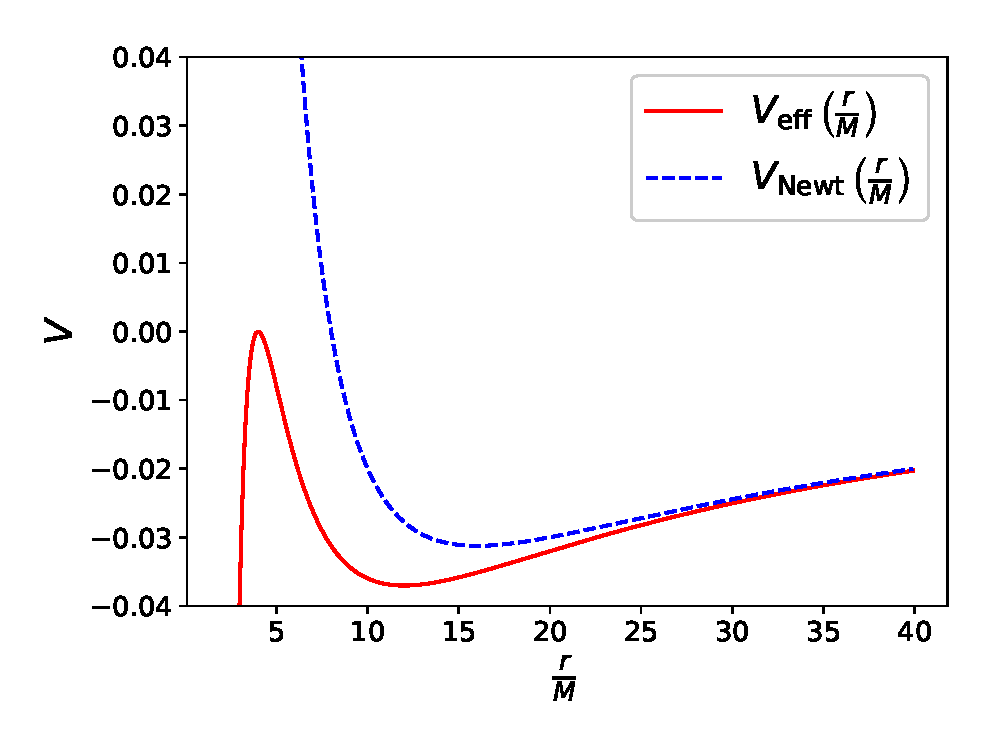
\includegraphics[width=\textwidth]{Figures/ch1/V_eff.eps}
        \end{figure}
    \end{minipage}
    \begin{minipage}{0.49 \textwidth}
        \begin{figure}
            \centering
            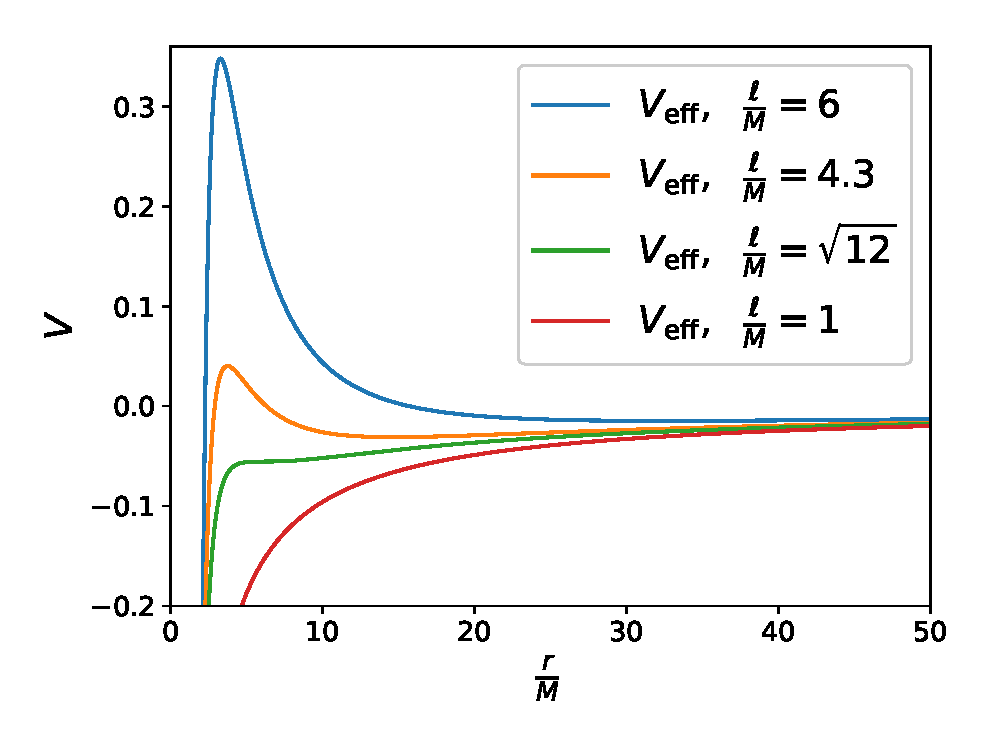
\includegraphics[width=\textwidth]{Figures/ch1/V_eff_tanti.eps}
        \end{figure}
    \end{minipage}

    \begin{equation*}
        V_{\rm eff}(r) = \frac{l^2}{2 r^2} - \frac{M}{r} - \frac{M l^2}{r^3}
    \end{equation*}

\end{frame}


\begin{frame}{Caduta Libera Radiale}

    Consideriamo $l = 0$, $\mathcal E = 0$, c'è una soluzione analitica

    \begin{figure}
        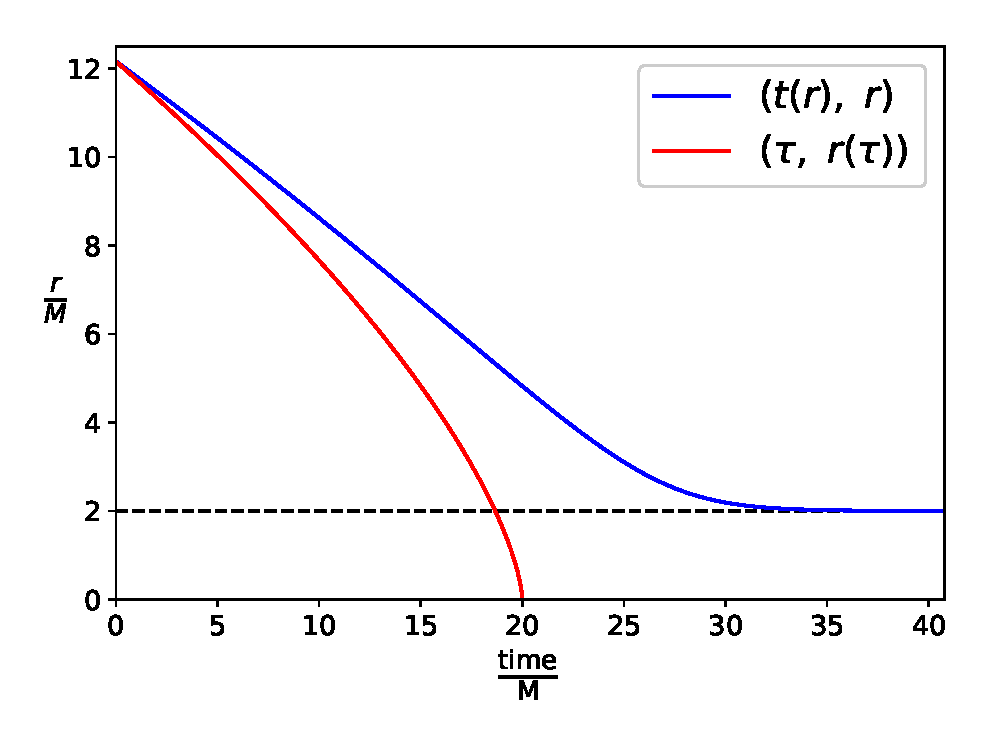
\includegraphics[width=0.53\textwidth]{Figures/ch1/radial_infall.eps}
    \end{figure}

    \begin{align*}
        r(\tau) &= \left(\frac{3}{2}\right)^{2/3}
        (2M)^{1/3} (\tau_* - \tau)^{2/3} \\
        t (r) &= t_* + 2M \left[ -\frac{3}{2} \left(\frac{r}{2M}\right)^{3/2}
        - 2 \left(\frac{r}{2M}\right)^{1/2}
        + \ln \abs{\frac{(r/2M)^{1/2} + 1}{(r/2M)^{1/2} - 1}} \right]
    \end{align*}

\end{frame}


\begin{frame}{$\mathcal E$ e Tipi di Orbita}

    \begin{equation*}
        \mathcal E = \frac{1}{2} \left( \dv{r}{\tau} \right)^2 + V_{\rm eff}(r, l)
    \end{equation*}

    \begin{figure}
        \centering
        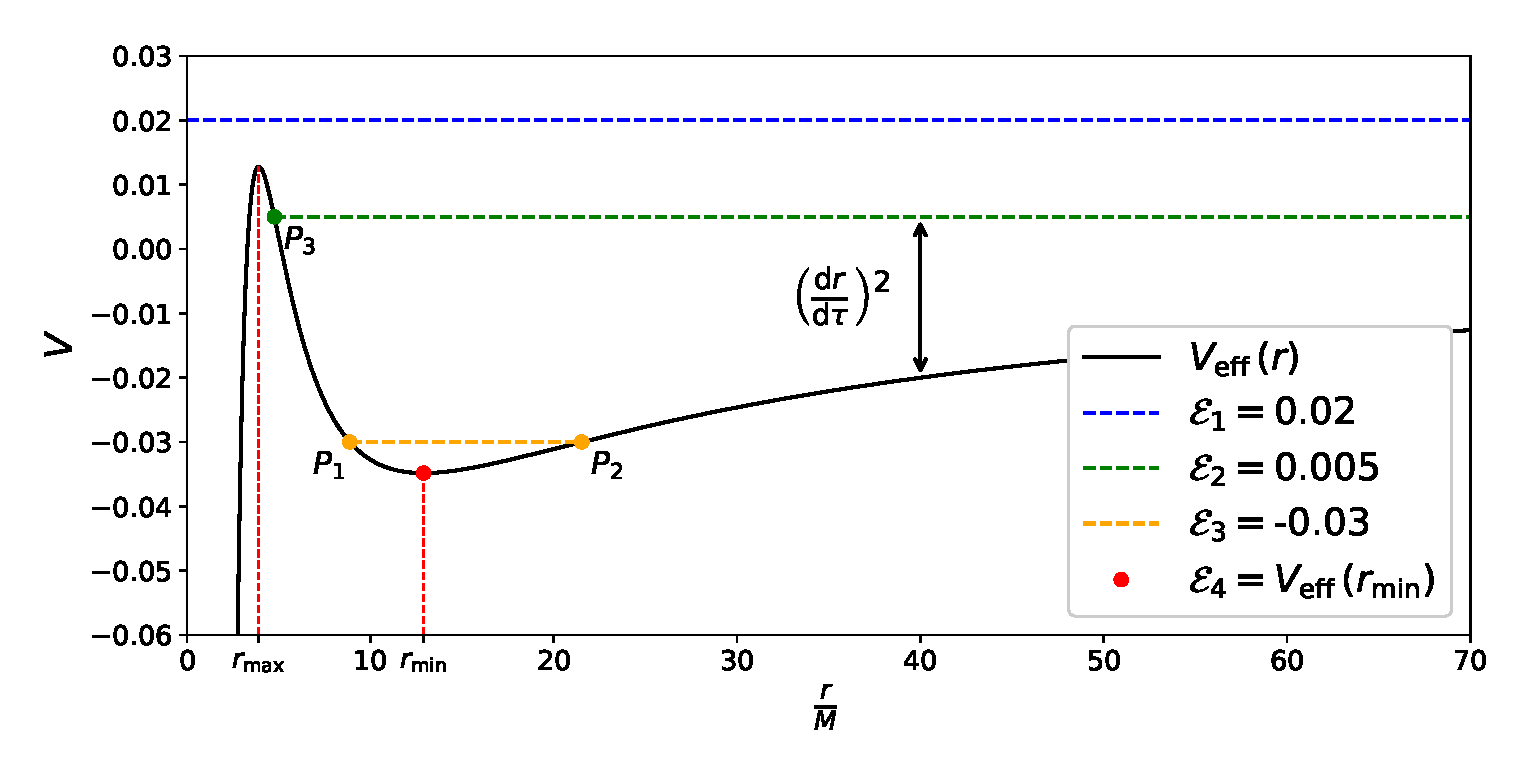
\includegraphics[width=\textwidth]{Figures/ch1/V_eff_orbits.eps}
    \end{figure}

\end{frame}


\begin{frame}{Orbite Stabili: Precessione}

    \begin{minipage}{0.4 \textwidth}
        \begin{figure}
            \centering
            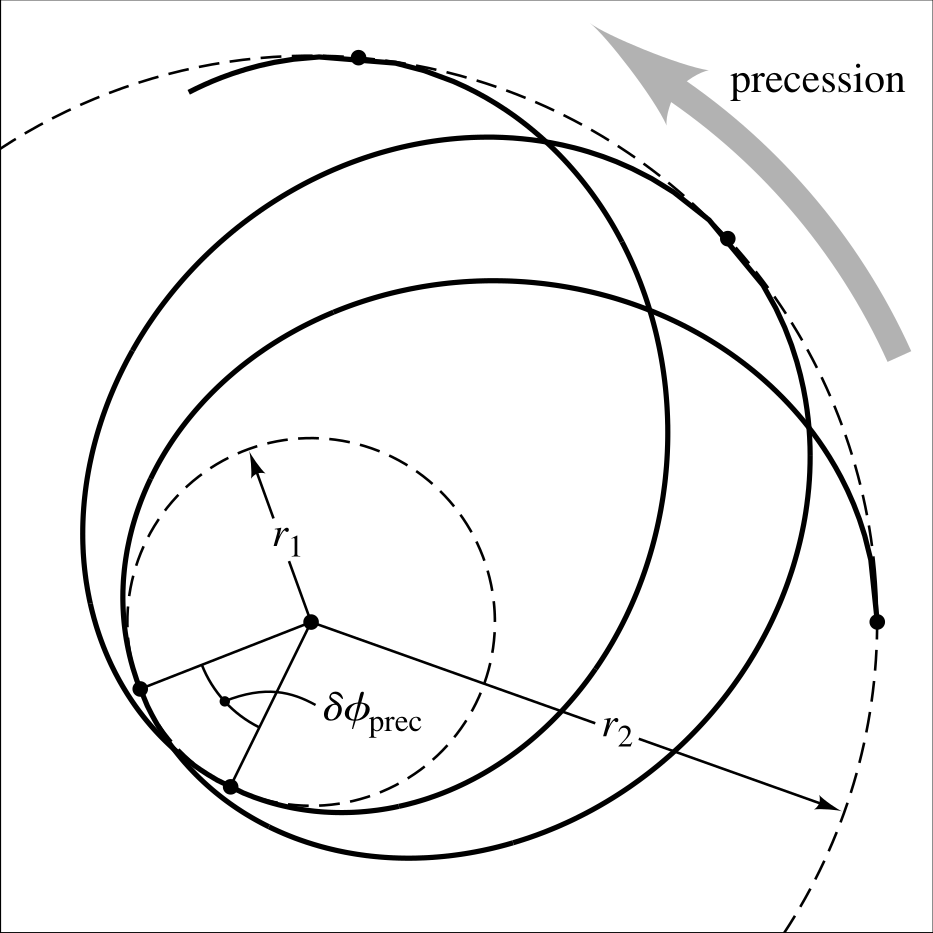
\includegraphics[width= 0.9 \textwidth]{Figures/ch1/precession_bozza.png}
            \caption{Da \textit{Gravity: An Introduction to Einstein's General Relativity, Hartle}}
        \end{figure}
    \end{minipage}
    \begin{minipage}{0.6 \textwidth}
        \begin{align*}
            \delta \phi &= \Delta \phi - 2 \pi \\ \\
            \dv{\phi}{\tau} &= \frac{\ell}{r^2} \\
            \dv{r}{\tau} &= \pm \sqrt{e^2 - \left(1 + \frac{\ell^2}{r^2}\right)
            \left(1 - \frac{2M}{r}\right)}
        \end{align*}
    \end{minipage}

    \begin{equation*}
        \Delta \phi = 2 \int_{r_1}^{r_2} \frac{\ell}{r^2}
        \left[e^2 - \left(1 + \frac{\ell^2}{r^2}\right)
        \left(1 - \frac{2M}{r}\right)\right]^{-1/2} \dd r
    \end{equation*}

\end{frame}


\subsection{Raggi di Luce}


\begin{frame}{Raggi di luce}

    Le uniche differenze sono la normalizzazione della velocità
    
    \begin{equation*}
        \mathbf{u \cdot u} = 0
    \end{equation*}

    e l'utilizzo di un parametro $\lambda$ al posto di $\tau$

    \begin{equation*}
        \dv{t}{\lambda} = \frac{e}{1 - \frac{2M}{r}} \quad \quad \quad
        \dv{\phi}{\lambda} = \frac{l}{r^2}
    \end{equation*}

    \begin{align*}
        \implies e^2 &= \left( \dv{r}{\lambda} \right)^2 + \ell^2 \,
        \underbrace{\frac{1}{r^2} \left( 1 - \frac{2M}{r} \right)}_{W_{\rm eff}} \\
    \end{align*}

\end{frame}


\begin{frame}{Il Parametro d'Impatto}

    \begin{equation*}
        \frac{e^2}{l^2} = \frac{1}{l^2} \left( \dv{r}{\lambda} \right)^2 + W_{\rm efff}
    \end{equation*}

    Grazie alla possibilità di ridefinire $\lambda \to l^2 \lambda$ possiamo
    scrivere

    \begin{equation*}
        \frac{1}{b^2} = \left( \dv{r}{\lambda} \right)^2 + W_{\rm eff}(r)
        \quad \quad \quad
        {\rm dove} \quad b = \abs{\frac{\ell}{e}}
    \end{equation*}

    \begin{figure}
    \centering
    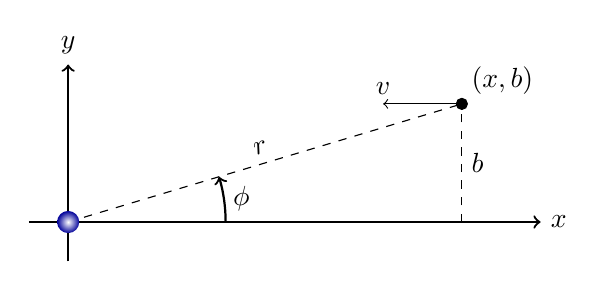
\begin{tikzpicture}

        % Cartesian axes
        \draw[thick,->] (-0.5,0) -- (6,0) node[right] {$x$};
        \draw[thick,->] (0,-0.5) -- (0,2) node[above] {$y$};

        % Particle at (x, d)
        \def\xP{5}
        \def\yP{1.5}
        \def\phiP{{atan(1.5 / 5)}}
        \filldraw[black] (\xP ,\yP) circle (2pt) node[anchor=south west] {$(x, b)$};

        % Draw the line r and d
        \draw[dashed] (0,0) -- (\xP, \yP) node[midway, above, sloped] {$r$};
        \draw[dashed] (\xP,0) -- (\xP, \yP) node[midway,right] {$b$};
        \draw[->] (\xP, \yP) -- (\xP - 1, \yP) node[above] {$v$};

        % Draw the angle theta
        \draw[thick,->] (2,0) arc [start angle=0,end angle=\phiP,radius=2cm];
        \node at (2.2,0.3) {$\phi$};

        % Star at origin (highlighted part)
        \shade[inner color=white, outer color=blue!60!black] (0,0,0) circle (4pt);

    \end{tikzpicture}
    \caption{Se $x \gg b$ allora $b$ è il parametro d'impatto}
    \end{figure}

\end{frame}


\begin{frame}{Il Potenziale Efficacie $W_{\rm eff}$}
    Ha solo un massimo $W_{\rm eff} (r = 3M) = \frac{1}{27 M^2}$

    \begin{figure}
        \centering
        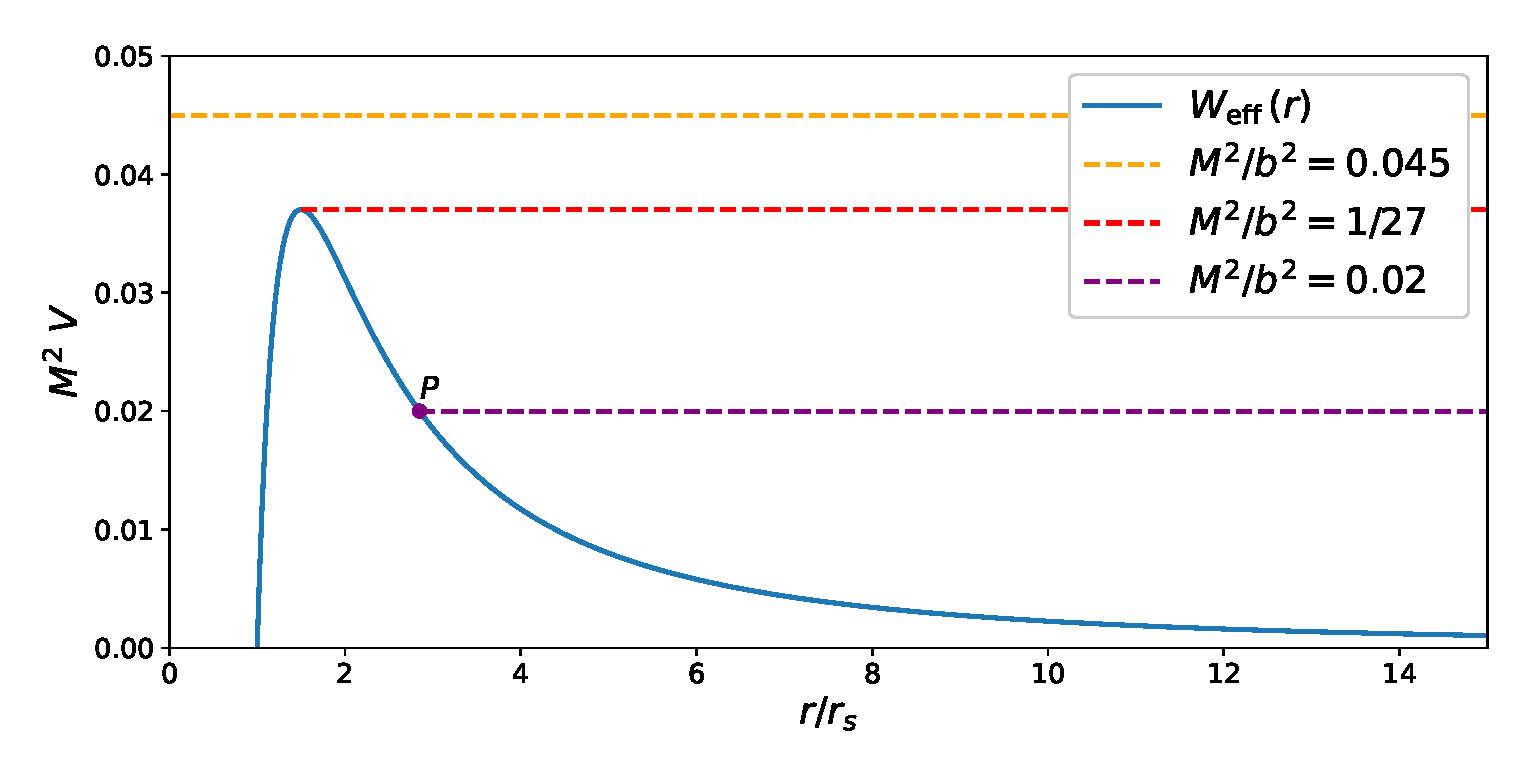
\includegraphics[width=0.9\textwidth]{Figures/ch1/W_eff_vs_b.eps}
    \end{figure}
    
    \begin{equation*}
        W_{\rm eff} (r) = \frac{1}{r^2} \left( 1 - \frac{2M}{r} \right)
    \end{equation*}

\end{frame}


\begin{frame}{Deflessione della Luce}

    \begin{equation*}
        \delta \phi = 2\int_{r_1}^\infty \frac{1}{r^2} \left[\frac{1}{b^2}
        - \frac{1}{r^2} \left(1 - \frac{2M}{r} \right) \right]^{-1/2} \mathrm{d}r
    \end{equation*}

    \begin{minipage}{0.49 \textwidth}
        \begin{figure}
            \centering
            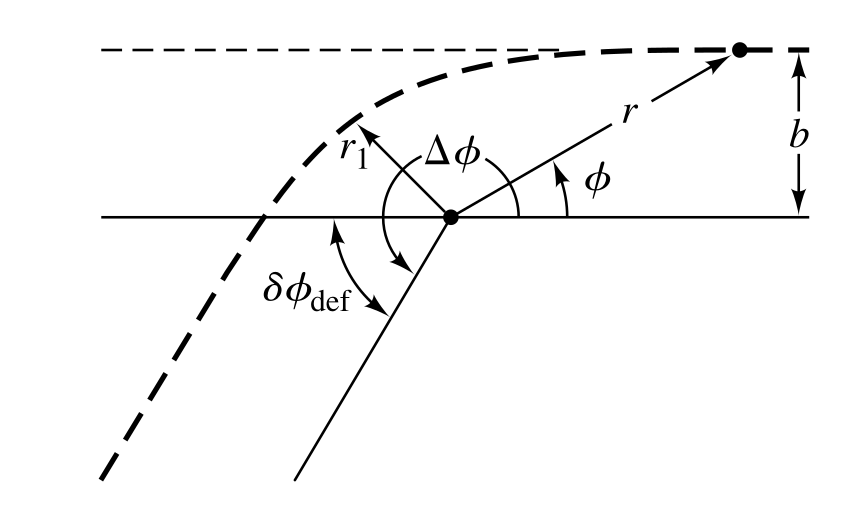
\includegraphics[width=\textwidth]{Figures/ch1/deflection.png}
            \caption{Da \textit{Gravity: An Introduction to Einstein's General Relativity, Hartle}}
        \end{figure}
    \end{minipage}
    \begin{minipage}{0.49 \textwidth}
        \begin{figure}
            \centering
            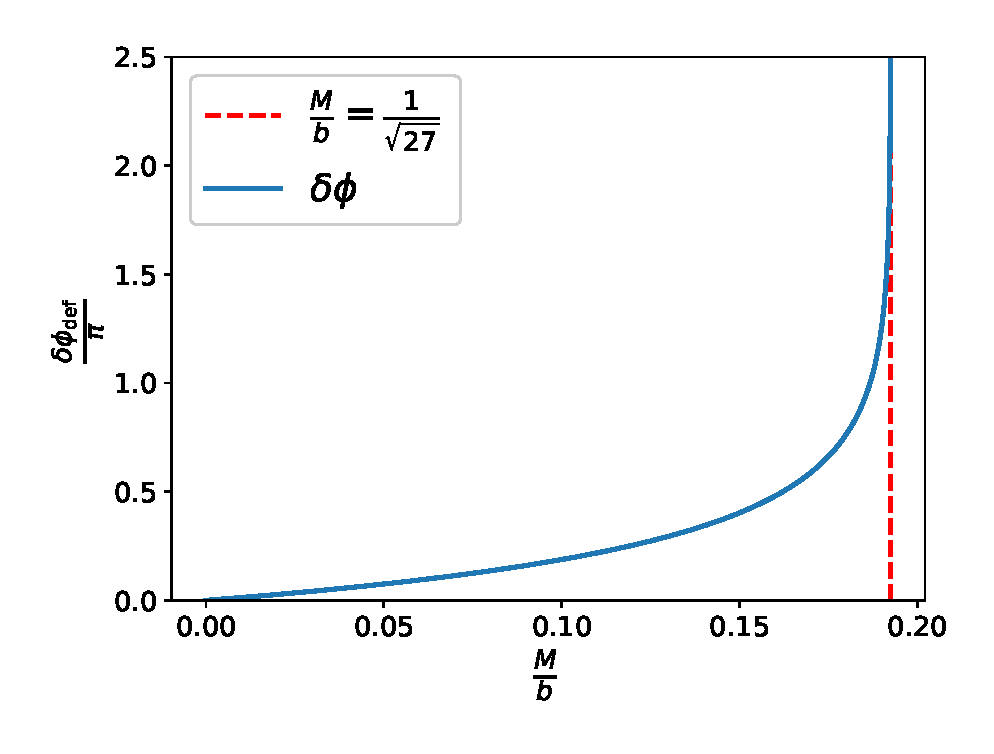
\includegraphics[width=\textwidth]{Figures/ch1/deflection_w.eps}
        \end{figure}
    \end{minipage}

\end{frame}
